
In KisTA is possible to model RTOS time services by means of \emph{schedulers}.
%
%
KisTA currently support the modelling of \emph{local schedulers}, that is,
schedulers which can handle a single processing element.
Only one scheduler can be mapped to a processing lement.
However, several application tasks can be mapped to a scheduler.

Schedulers can be configured wid different scheduling policies.
Three main parameters can be configured for each scheduler instance:

\begin{itemize}
\item \textbf{Time Slicing:} states if the scheduler considers a tick timer event to perform a scheduling
\item \textbf{Preemption Policy:} states if the scheduler can preempt or not a task currently running upon a
communication event (which can modify the list of tasks ready to execute). 
In case or enabling a tick timer event, then a preemptive policy will make possible a pre-emption
after a scheduling provoked by a tick timer event.
\item \textbf{Scheduling policy}:States which tasks assigned to the local scheduler, among the tasks
in a ready-to-execute state, will be running right after the schedule.
\end{itemize}

For the time slicing attribute, the user can state if there is time slicing or not. 
The user can also configure also the tick timer time.

Regarding the preemption Policy, the user can state if the scheduler is pre-emptive or not.

The user has serveral possibilities regarding the dispatching policy.
KisTA supports the following possibilities:
\begin{itemize}
\item Static Scheduling
\item Cycle Executive
\item Static priorities: 
\item Dynamic priorities
\end{itemize}

Additional attributes are required depending on the dispatch policy.
Static scheduling requires to provide the static schedule, i.e. the order of execution of
the tasks assigned to the scheduler.
Static priorities based scheduling required to sate the priorities (user defined, rate-monotonic, deadline monotonic, density monotonic).
Currently, the EDF dynamic scheduling policy is supported.
%
In order to avoid capturing all the attributes for wide-spread policies,
e.g., rate-monotonic, EDF, etc, KisTA provides shorcuts, for a synthetic description of them.

In addition, KisTA supports the description of the communication scheduling policy.
This policy is also described on the SW platform lawer. 
Currently supports FIFO with priority communication scheduling.

\subsection{Using the C/C++ API}
TBC


\subsection{Using the XML-Front end}
TBC

The Listing~\ref{list:xml_sched_edf} shows an excerpt of the system description
in the \texttt{\$KISTA/examples/xml\_if/basic\_real\_time/brt\_ex5}.
This example describes the same system as in the 
\texttt{\$KISTA/examples/basic\_real\_time/brt\_ex5} folder,
but describing the system in XML, using the KisTA XML front-end.
%
Specifically, the excerpt shows how to describe the scheduler \emph{sched1},
configuring it 
configure to only export the image and scaling up 25\% the original size.
The resulting sketch is shown in Figure~\ref{fig:vad_sketch_only_img_1_25}.

%\begin{table}[t]
\begin{lstlisting}[language=XML, caption={Describing a scheduler with EDF policy.}, label=list:xml_sched_edf]
  <SW_platform>
    <rtos name="sched1">
      <!--tasks scheduling -->
      <task_scheduler>
        <scheduler_policy policy="dynamic_priorities"
                          triggering="preemptive"
                          time_slice="no">
          <dispatching value="EarliestDeadlineFirst" />
        </scheduler_policy>

      </task_scheduler>
      <!--
	  <tick_timer value="10" unit="ms"/>
         -->  
    </rtos>
  </SW_platform>
\end{lstlisting}

The Listing~\ref{list:xml_sched_edf_short} shows the short mechanism to make the same description.

%\begin{table}[t]
\begin{lstlisting}[language=XML, caption={Describing a scheduler with EDF policy.}, label=list:xml_sched_edf_short]
  <SW_platform>
    <rtos name="sched1">
      <scheduler_policy  policy="EDF"/>
    </rtos>
  </SW_platform>
\end{lstlisting}

Figure~\ref{fig:brt5_xml_trace} shows the trace with the state of the
tasks and of the scheduler \emph{sched1}, once the description of the system
has been done in XML, and once the functionality is linked to this
description via the task wrapper functions.

It can be seen how the result is the same.


\begin{figure}[h]
\centering
%\includegraphics[width=\textwidth]{./figs/.png} 
\fbox{
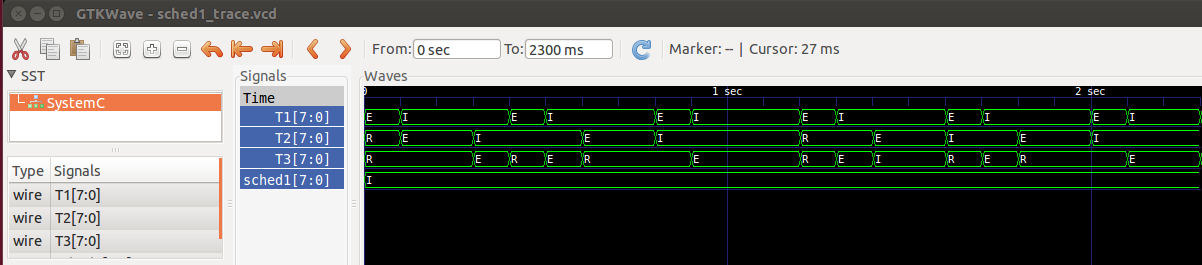
\includegraphics[width=0.9\textwidth]{./figs/brt5_xml_trace.png} 
}
\caption{Trace of the BRT5 example, with three tasks and EDF scheduling.} 
\label{fig:brt5_xml_trace}
\end{figure}
